\chapter{The OSI Model and TCP/IP
Suite}\label{the-osi-model-and-tcpip-suite}

\section{What is a networking model?}\label{what-is-a-networking-model}

Networking models categorize and provide a structure for networking
protocols and standards.

(Protocols are a set of logical rules defining how network devices and
software should work)

\section{OSI MODEL}\label{osi-model}

\begin{itemize}
\tightlist
\item
  Open Systems Interconnection Model
\item
  Conceptual model that categorizes and standardizes the different
  functions in a network.
\item
  Created by the ``International Organization for Standardization''
  (ISO)
\item
  Functions are divided into 7 ``Layers''
\item
  These layers work together to make the network work.
\end{itemize}

\begin{figure}
\centering
\pandocbounded{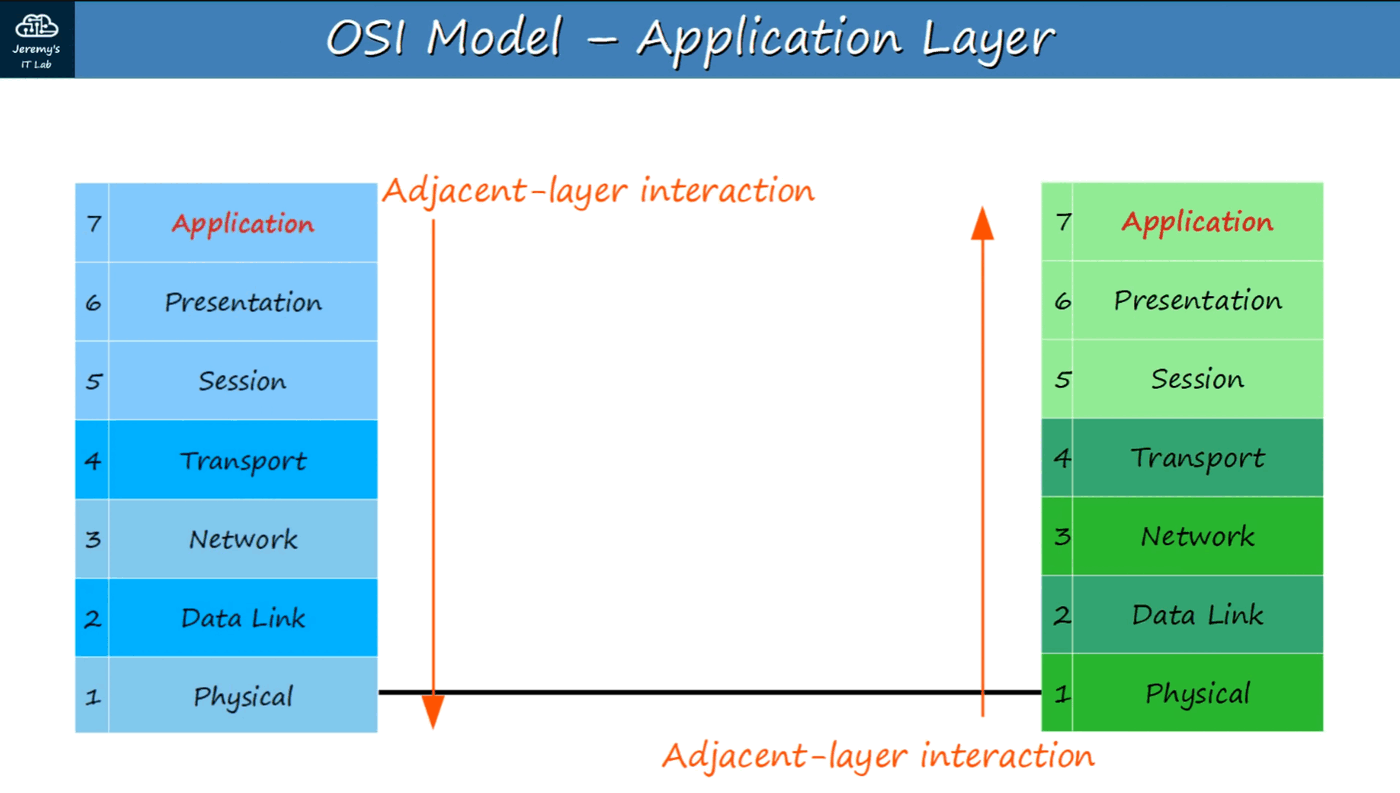
\includegraphics[keepaspectratio,alt={image}]{images/03-osi-model-tcpsuite/img-001.png}}
\end{figure}

As data moves from the top layer, downward, the process is called
``encapsulation''

As data moves from the bottom layer, upward, the process is called
``de-encapsulation''

When interactions occur on the same layer, it's called ``same-layer
interaction''

\begin{figure}
\centering
\pandocbounded{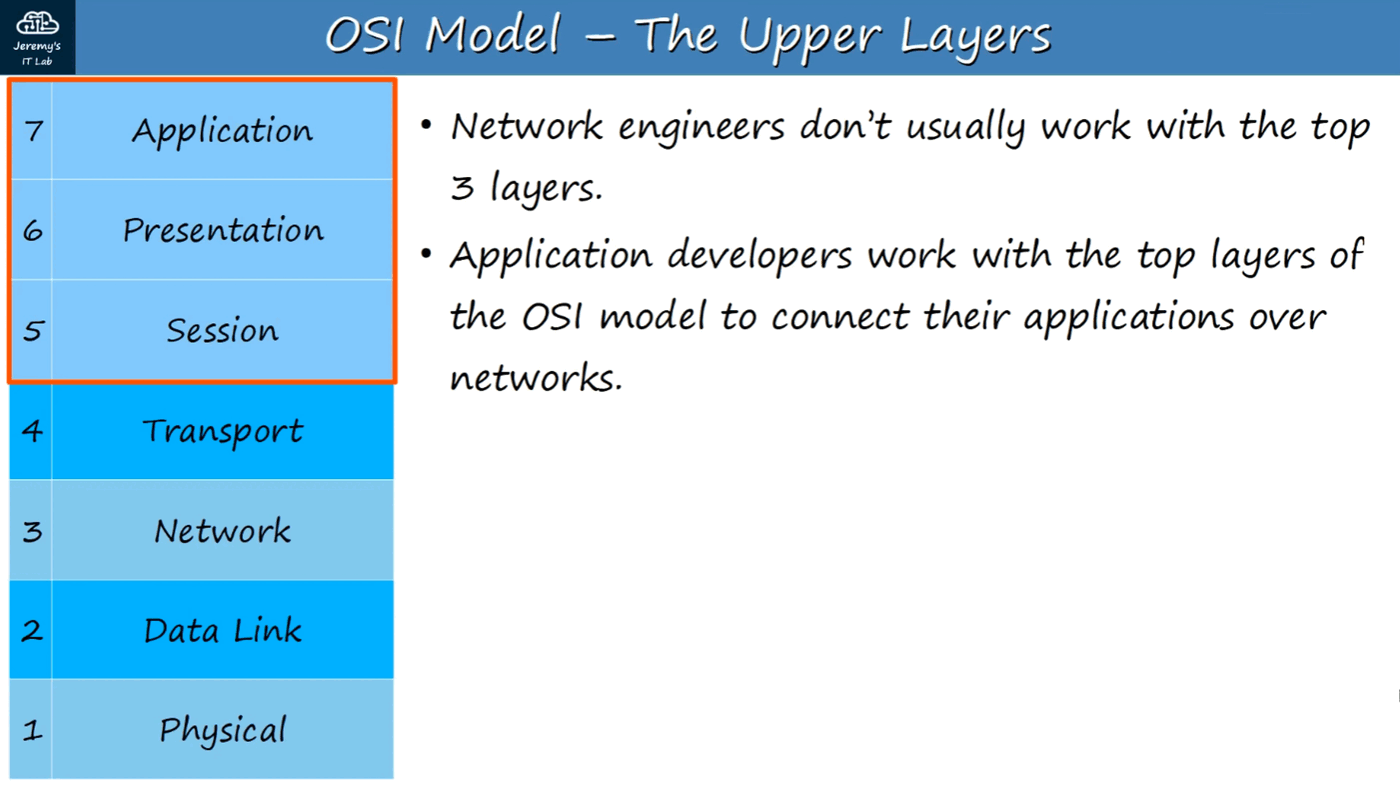
\includegraphics[keepaspectratio,alt={image}]{images/03-osi-model-tcpsuite/img-002.png}}
\end{figure}

Mnemonic to help remember the Data Layer Names / Order

\begin{figure}
\centering
\pandocbounded{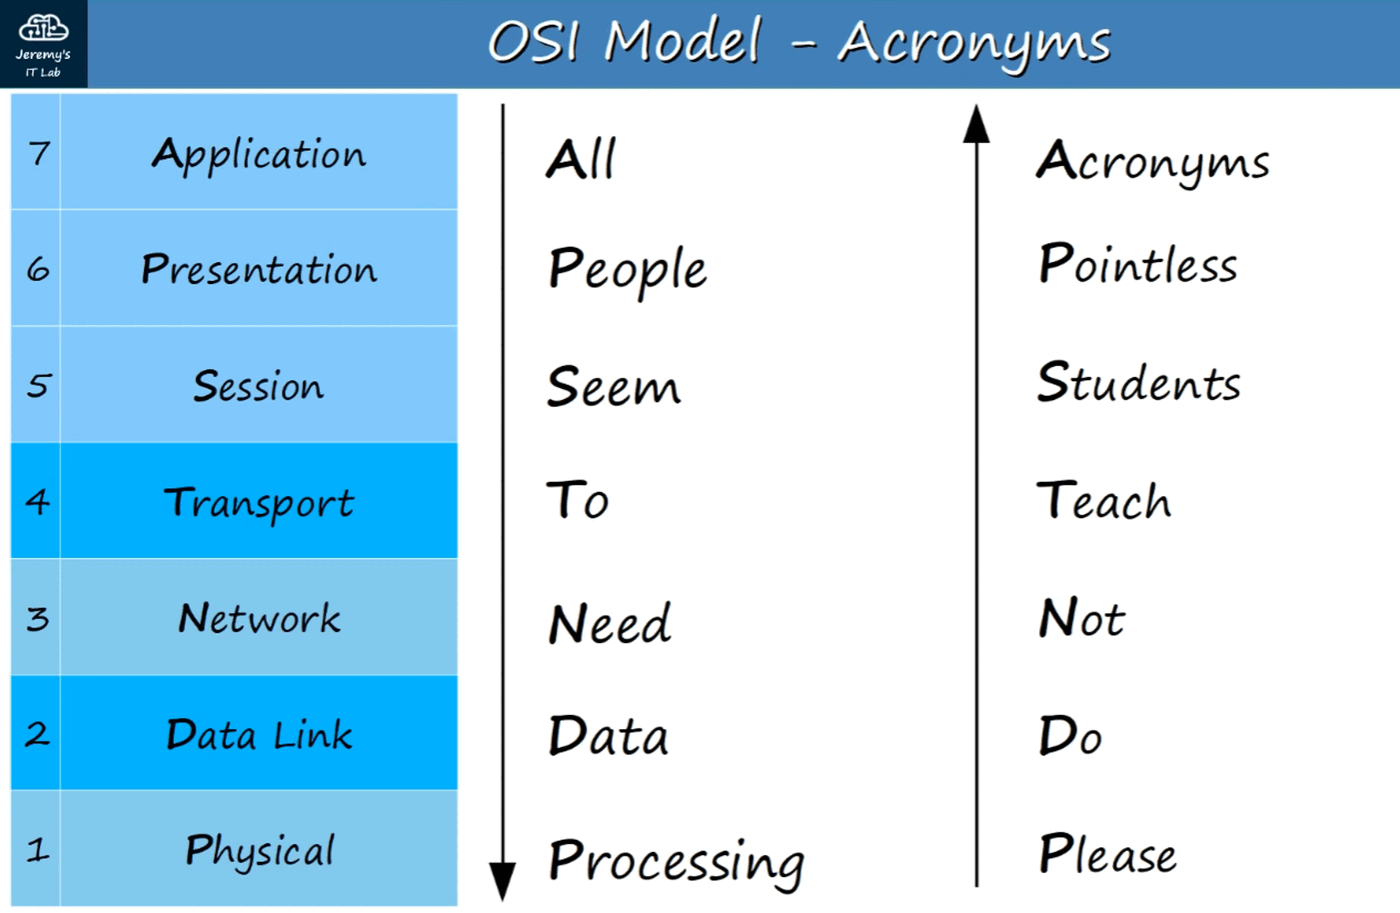
\includegraphics[keepaspectratio,alt={image}]{images/03-osi-model-tcpsuite/img-003.png}}
\end{figure}

\subsection{The layers are :}\label{the-layers-are}

\subsection{7 - APPLICATION}\label{application}

\begin{itemize}
\tightlist
\item
  This Layer is closest to end user.
\item
  Interacts with software applications.
\item
  HTTP and HTTPS are Layer 7 protocols
\end{itemize}

Functions of Layer 7 include:

\begin{itemize}
\tightlist
\item
  Identifying communication partners
\item
  Synchronizing communication
\end{itemize}

\subsection{6 - PRESENTATION}\label{presentation}

\begin{itemize}
\tightlist
\item
  Translates data to the appropriate format (between Application and
  Network formats) to be sent over the network.
\end{itemize}

\subsection{5 - SESSION}\label{session}

\begin{itemize}
\tightlist
\item
  Controls dialogues (sessions) between communicating hosts.
\item
  Establishes, manages, and terminates connections between local
  application and the remote application.
\end{itemize}

Network engineers don't usually work with the top 3 layers. Application
developers work with the top layers of the OSI model to connect their
applications over networks.

\subsection{4 - TRANSPORT}\label{transport}

\begin{itemize}
\tightlist
\item
  Segments and reassembles data for communication between end hosts.
\item
  Breaks large pieces of data into smaller segments which can be more
  easily sent over the network and are less likely to cause transmission
  problems if errors occur.
\item
  Provides HOST-TO-HOST (end to end) communication
\end{itemize}

When Data from Layer 7-5 arrives, it receives a Layer 4 Header in the
Transport layer.

\textless\textless{} DATA + L4 Header \textgreater\textgreater{}

This is called a SEGMENT.

\subsection{3 - NETWORK}\label{network}

\begin{itemize}
\tightlist
\item
  Provides connectivity between end hosts on different networks (ie:
  outside of the LAN).
\item
  Provides logical addressing (IP Addresses).
\item
  Provides path selection between source and destination
\item
  \textbf{ROUTERS} operate at Layer 3.
\end{itemize}

When Data and the Layer 4 Header arrive in the Network Layer, it
receives a Layer 3 Header.

\textless\textless{} DATA + L4 Header + L3 Header
\textgreater\textgreater{}

This is called a \textbf{PACKET}.

\subsection{2 - DATA LINK}\label{data-link}

\begin{itemize}
\tightlist
\item
  Provides NODE-TO-NODE connectivity and data transfer (for example, PC
  to Switch, Switch to Router, Router to Router)
\item
  Defines how data is formatted for transmission over physical medium
  (for example, copper UTP cables)
\item
  Detects and (possibly) corrects Physical (Layer 1) errors.
\item
  Uses Layer 2 addressing, separate from Layer 3 addressing.
\item
  \textbf{SWITCHES} operate at Layer 2
\end{itemize}

When the Layer 3 Packet arrives, a Layer 2 Trailer and Header are added.

\textless\textless{} L2 Trailer + DATA + L4 Header + L3 Header + L2
Header \textgreater\textgreater{}

This is called a FRAME.

All the steps leading up to transmission is called ENCAPSULATION. When
the frame is sent to the receiver, it then goes through the reverse
process, DE-ENCAPSULATION, stripping off layers while travelling from
OSI Layer 1 to Layer 7.

\subsection{1 - PHYSICAL}\label{physical}

\begin{itemize}
\tightlist
\item
  Defines physical characteristics of the medium used to transfer data
  between devices. For example : voltage levels, maximum transmission
  distances, physical connectors, cable specs.
\item
  Digital bits are converted into electrical (for wired connections) or
  radio (for wireless connections) signals.
\item
  All of the information in SECTION 2 (NETWORKING DEVICES) is related to
  the Physical Layer
\end{itemize}

\subsection{OSI MODEL - PDU's}\label{osi-model---pdus}

\begin{figure}
\centering
\pandocbounded{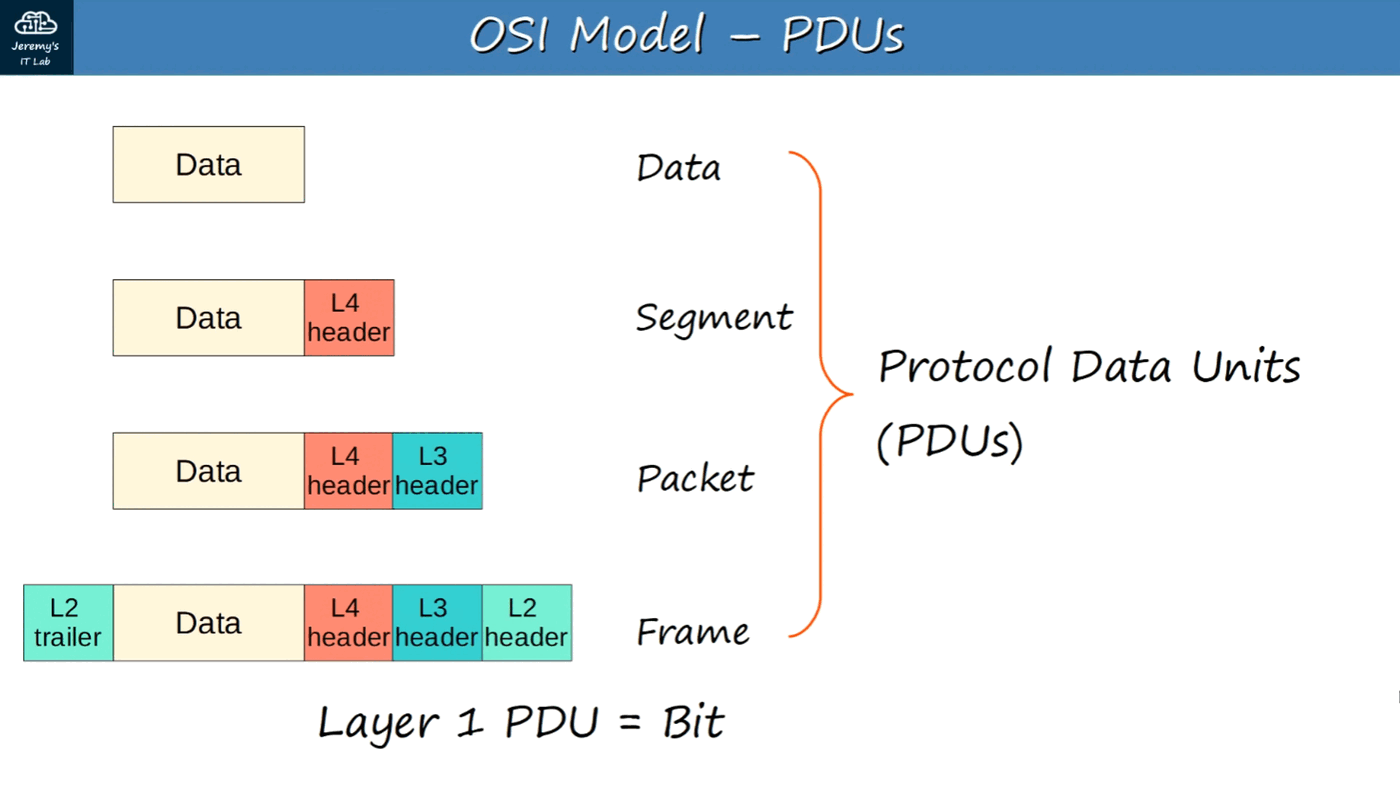
\includegraphics[keepaspectratio,alt={image}]{images/03-osi-model-tcpsuite/img-004.png}}
\end{figure}

A PDU is a Protocol Data Unit. Each step of the process is a PDU.

{\def\LTcaptype{none} % do not increment counter
\begin{longtable}[]{@{}lll@{}}
\toprule\noalign{}
OSI LAYER \# & PDU NAME & PROTOCOL DATA ADDED \\
\midrule\noalign{}
\endhead
\bottomrule\noalign{}
\endlastfoot
7-5 & DATA & Data \\
4 & SEGMENT & Layer 4 Header Added \\
3 & PACKET & Layer 3 Header Added \\
2 & FRAME & Layer 2 Trailer and Header Added \\
1 & BIT & 0s and 1s Transmission \\
\end{longtable}
}

\textless\textless{} L2 Trailer + DATA + L4 Header + L3 Header + L2
Header \textgreater\textgreater{}

\subsection{TCP/IP Suite}\label{tcpip-suite}

\begin{itemize}
\tightlist
\item
  Conceptual model and set of communications protocols used in the
  Internet and other networks.
\item
  Known as TCP/IP because those are two of the foundational protocols in
  the suite.
\item
  Developed by the US Dept. of Defense through DARPA (Defense Advanced
  Research Projects Agency).
\item
  Similar structure to the OSI Model, but fewer layers.
\item
  THIS is the model actually in use in modern networks.
\item
  \begin{itemize}
  \tightlist
  \item
    Note : The OSI Model still influences how network engineers think
    and talk about networks.
  \end{itemize}
\end{itemize}

\begin{figure}
\centering
\pandocbounded{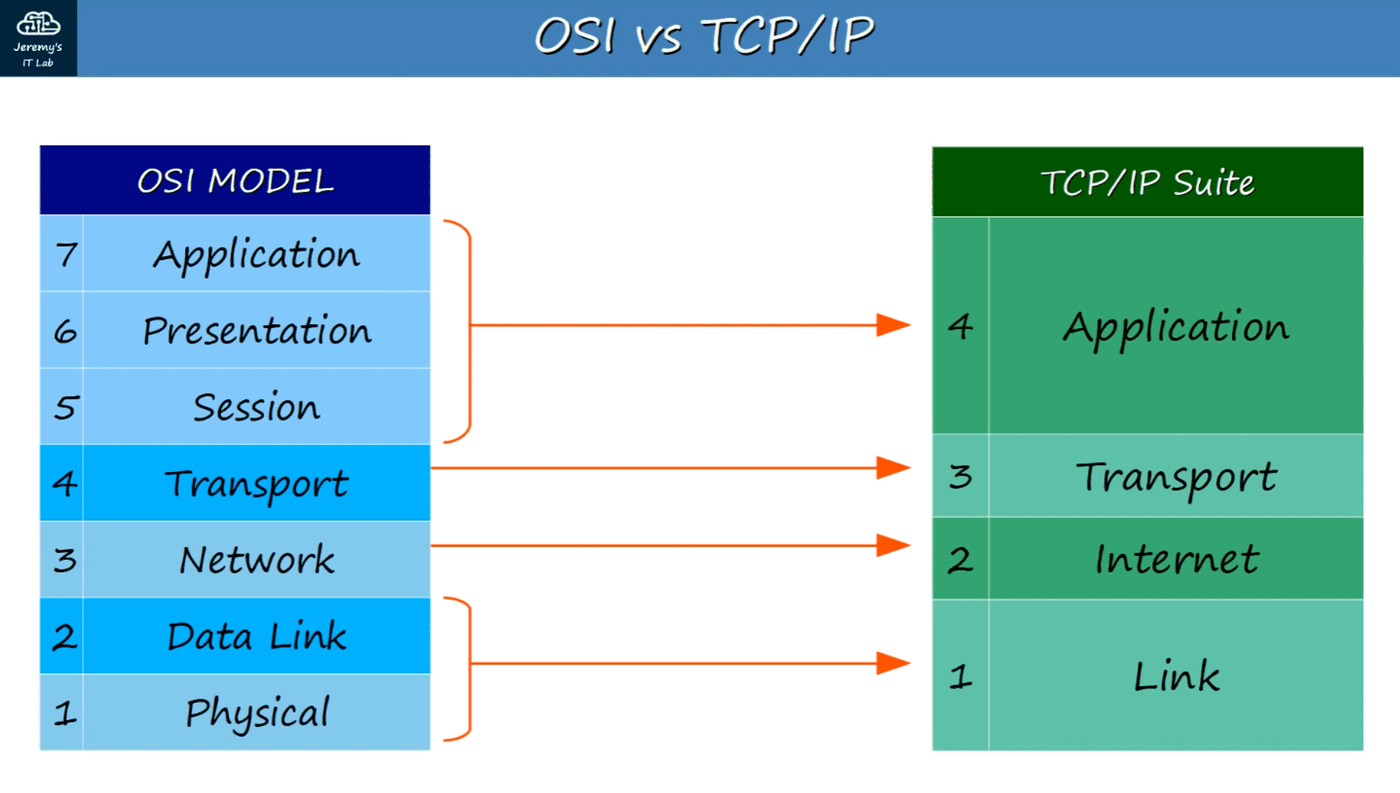
\includegraphics[keepaspectratio,alt={image}]{images/03-osi-model-tcpsuite/img-005.png}}
\end{figure}

\subsection{Layer Interactions}\label{layer-interactions}

\begin{figure}
\centering
\pandocbounded{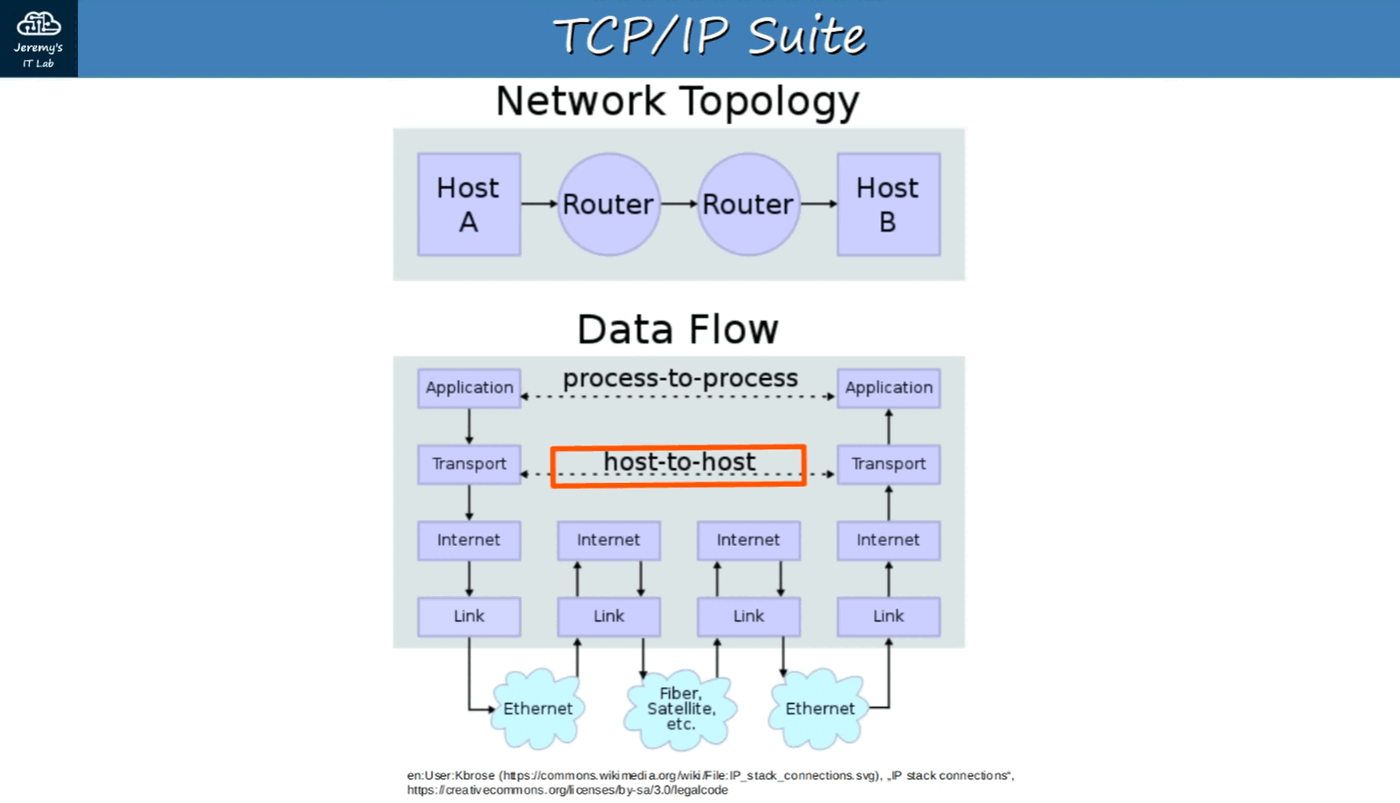
\includegraphics[keepaspectratio,alt={image}]{images/03-osi-model-tcpsuite/img-006.png}}
\end{figure}

Adjacent-Layer Interactions:

\begin{itemize}
\tightlist
\item
  Interactions between different layers of the OSI Model on same host.
\end{itemize}

Example:

Layers 5-7 sending Data to Layer 4, which then adds a Layer 4 header
(creating a SEGMENT).

Same-Layer Interactions:

\begin{itemize}
\tightlist
\item
  Interactions between the same Layer on different hosts.
\item
  The concept of Same-Layer interaction allows you to ignore the other
  layers involved and focus on the interactions between a single layer
  on different devices.
\end{itemize}

Example:

The Application Layer of YouTube's web server and your PC's browser.
